 %!TEX root=title.tex
\section{Social Weaver - Conceptual Level}\label{sowe-abstract}

\epigraph{I know it when I see it}{Potter Stewart}

Even though Stewart had something slightly different in mind when he used this famous phrase in front of the  United States Supreme Court, it is still a quite good explanation why a prototype is useful. 

We aim to create a vertical prototype. That means that our system should proof that the general idea is possible to implement. Wiegers writes that a vertical prototype should touch all technical layers to serve as a \emph{proof of concept}\cite{wiegers2003software}.

First of all we start with a prototype driven requirements analysis. In Section \ref{what_is_sowe} \nameref{what_is_sowe} we discuss the requirements on a conceptual level and put these into a relationship with the \emph{WHY/WHAT/WHO-Model} \cite{van2009requirements}.

Based on that in Section \ref{sowe-concrete} we bring the requirements to a implementation level and furthermore explain some interesting details about the derived architecture and implementation. 

\subsection{The WHY-WHAT-WHO-Model}\label{why-what-who}
\begin{figure}\centering
		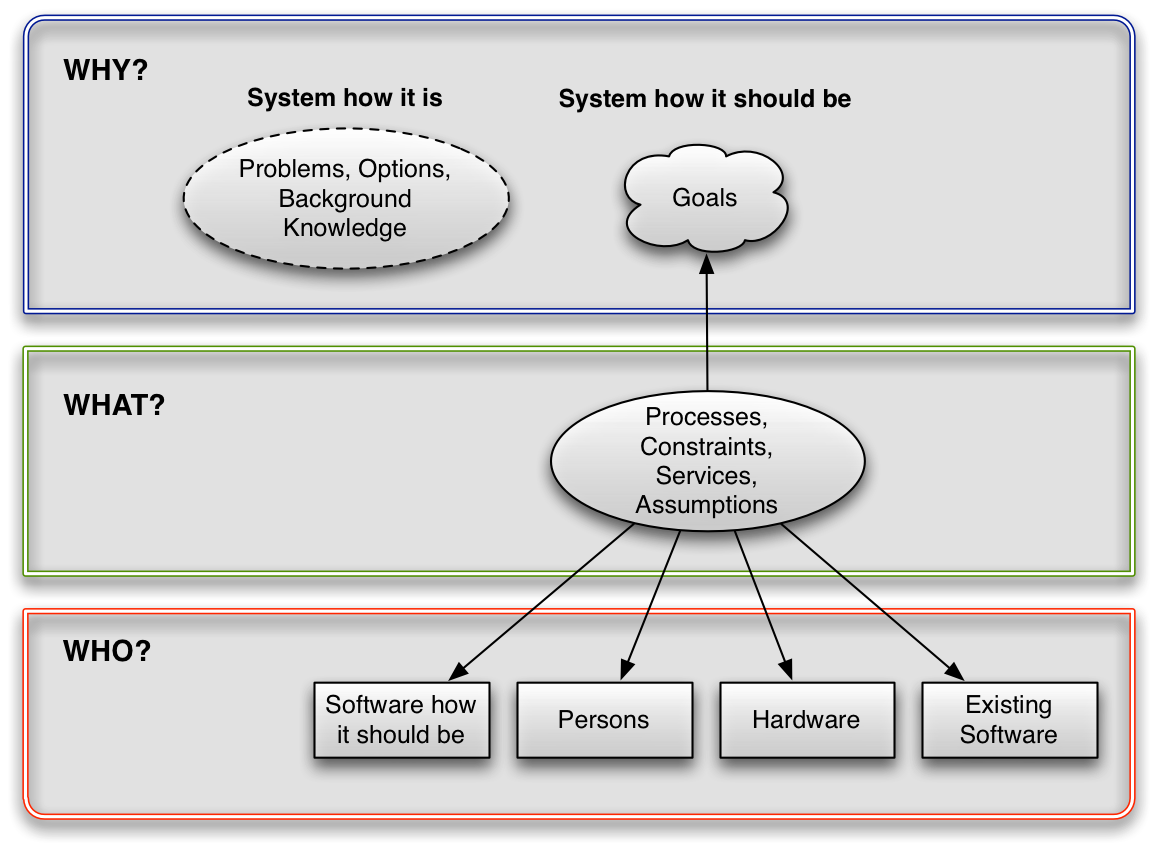
\includegraphics[width=10cm]{images/why-what-who-model.png}
		\caption{Three dimensions of the requirements types \cite{van2009requirements}}
		\label{why-what-who-diagram}
\end{figure} 

The WHY-WHAT-WHO model (see Figure \ref{why-what-who-diagram}) enables us to discuss on different layers of requirements abstraction. The purpose of the WHY-WHAT-WHO model should not be a strict separation into sections. It is much more to be seen as a context that we can refer to through this paper.

In the following all layers are described in detail and connected to parts of this thesis. 

\subsubsection{WHY Dimension}
This dimension analyses the existing system or environment 
we build on, to define what is within a possible reach. Potential problems or limitations should be defined in context of this layer. Furthermore we should try to see what impact our system is going to have on the environment. 

For this task we first of all need background knowledge which we gather in a domain analysis. Based on that we are be able to define the problem, that should be our motivation for building such a system. 

\nameref{domainAnalysis} \ref{domainAnalysis} is related to the WHY dimension.

\subsubsection{WHAT Dimension}

The WHAT dimension contains services, constraints and processes that are direct results from the WHY dimension and lead to the actual goal system. At this point the results from the WHY dimension should be verified if they are still applicable and possible to implement. Use Cases and concrete requirements belong to this section. 

This thesis Sections \ref{sowe-reqs} \nameref{sowe-reqs} and \ref{usecases} \nameref{usecases} are related to the WHAT dimension.

\subsubsection{WHO Dimension}

The WHO dimension is about distinguishing what component has which responsibility. Components in this context don't need to be necessarily hardware components. For instance, some user interaction might be classified as component. Responsibility in this context means that the component achieves the objectives (\cite{van2009requirements}).

This dimension is not applicable to certain sections. Throughout the thesis it becomes obvious what components have what functions to achieve objectives. 

As example imagine the process of weaving a social element to a web view. It includes several components:
\begin{itemize}
	\item User
	\item Plugin
	\item Web Service
	\item Browser
	\item Web view
\end{itemize}

The users interaction is needed to determine the correct web view within the browser. The browser initiates the plugin, whereupon the plugin uses information about the web view, that is provided by the browser, to create content, that is transmitted to the server. 

\newpage
\subsection{Domain Analysis}\label{domainAnalysis}

\begin{enumerate}[A.]
\item Introduction\\
The domain analysis contains gathered knowledge about using web applications or web pages and that is related to Social Weaving. This already established environment provides more knowledge that we need for the analysis. We  need to generalize it and additionally create new knowledge about Social Weaving, including meanings of processes and definition of terms. With this as root position we are be able to create requirements and define use cases. 
	
\item Glossary
\begin{description}
	\item[Web view] describes the environment that is visible withing a browser. It may be a web application, a web page or any other displayed HTML code processed by the browser. In the context of social weaving the back end code is is not an issue at all. 
	
	\item[Social element] is some user generated content that is weaved into the web view. It is called social element because it provides some kind of collaboration possibilities. This can be a chat, comment box, file upload or just a link to external content.
	
	\item[Social Weaving] we call the whole process of weaving some social content into a web view. 
\end{description}
	
\item General knowledge about the domain\\
\begin{itemize}
	\item Recognizing web elements in web views across sessions is a problem
	\item Web page and application architectures differ a lot
	\item Web views evolve with time
	\item User is able to uniquely identify elements in a web view
	\item Some web technologies cannot be analyzed (Flash, Shockwave, ...)
\end{itemize}

\item Clients\\
First of all we distinguish between the types of clients: user and administrators. Even though this as technical domain analysis to support the prototype development process, additionally some categories of possible users types are mentioned. This should give the reader an idea about possible real world use cases. 
\begin{itemize}
	\item User \\ 
		Basically, any browser users is a potential client. All that is required besides the browser itself is a compatible plugin that supports Social Weaving. 
		\begin{itemize}
			\item Client \& Consultant \\
			The client is using a platform (like ERP or banking system) and might ask his consultant directly posting his question in the view and location where the problem seems to be. The consultant answers directly in place. Both users have different roles. The client, for instance, can only post questions and not see the question of other users. Consultants can only answer and see all questions of all clients.
			\item Collaboration in Teams\\
			Several users have a communally sessions. All users can add, modify and see the social elements. This use case is useful, for example, when a consultant team works with a system. Questions and other kind of communication is persisted directly to the relevant items in the view.
		\end{itemize}
	\item Administrator\\
	Every Social Weaving session needs an administrator who configures and keeps the web service running. Theoretically this can be also a regular user. Nevertheless this role has to be maintained to make a synchronization between user session possible. 
\end{itemize}
	
\item Environment\\
For the prototype environment all users need to have a working computer with the Firefox browser and an installed plugin.  Additionally the web service needs to be running on a Tomcat server. 

A future goal is to support more browsers but is not covered in this thesis. 

\item Similarity to other software\\
There is no known software that performs Social Weaving. Anyway the basic idea of annotating something is not new. Many systems provide the possibility of commenting. For instance, task managers like Asana\footnote{\url{http://asana.com/}} or agile platforms like \footnote{\url{http://www.jetbrains.com/youtrack/}} provide flexible possibilities to comment a lot of things and upload files in any text field. Nevertheless it is not possible to annotate something that is not meant to be accessible. 

Another analogical case of Social Weaving is annotation documents. There are many tools out there that you can use to annotate PDF files with comments, icons and links. Compared to task mangers, we discussed above, here it is possible to annotate basically anything within the document. But still this is pretty much different from annotating any web view. 

\item Similarity to other software domains\\
The idea to analyze web pages or web applications by its source code (meaning both server as well as client side generated HTML code) is not new. Some of these approaches were used as inspiration for the Social Weaving approach. 
First of all we discuss the rudiments to some comparable domains; afterwards the differences are explained and how Social Weaving differs from already existing work.
	\paragraph{Web Site Re-engineering Using RMM}\mbox{}\\
	
	\begin{figure}\centering
			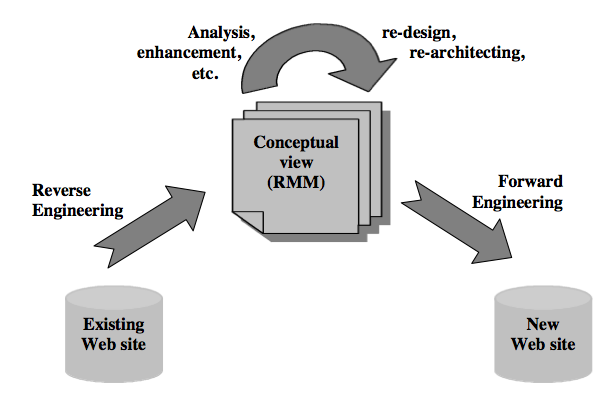
\includegraphics[width=10cm]{images/rmm-phases.png}
			\caption{Web site reengineering phases. \cite{antoniol2000web}}
			\label{rmm-phases}
	\end{figure} 
	
	The goal of this technique is to re-design exisiting web pages to a new and structured architecture, so they can be reused for similar cases. Basically, the reengineering process consists of the following steps (also shown in Figure: \ref{rmm-phases}):
	
	\begin{enumerate}
		\item Reverse Engineering\\
			The conent of the web page is processed for further analysis.
		\item Analysis\\ 
			The current content is recovered into a Relationship Management Methodolgy (RMM) design.
		\item Re-Design\\
			The recovered design is used to form the web site file into an Relational Database Management System.
		\item Forward engineering\\
			New web site can be created using the re-designed data from database.
	\end{enumerate}
	
	This approach was proposed as paper for the Reengineering Week 2000 in Zurich \cite{antoniol2000web}. Unfortunately there doesn't seem to be implementation or sample case for this study. 

	\begin{figure}\centering
			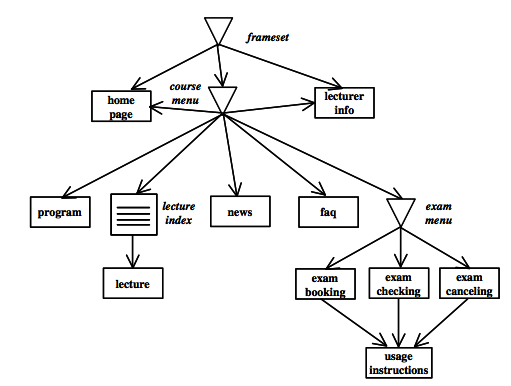
\includegraphics[width=9cm]{images/rmm-example.png}
			\caption{Example for RMM. It is related to the scenario that can be found in \cite{antoniol2000web}}
			\label{rmm-example}
	\end{figure} 
	\begin{description}
	
		\item[\emph{RMM}]\mbox{}\\
		Relationship Management Methodolgy is supposed to support design and implementation of web sites that are based on relational databases. Its core is based on the Entity Relationship (ER) model, which is commonly used in the context of relational databases \cite{batini1992conceptual}. An example for a RMM diagram can be seen in Figure \ref{rmm-example}. 
		
		\item[\emph{Comparison}]\mbox{}\\
		Even though the goals of Social Weaving and reengineering with the RMM technique are quite different, both approaches has to deal with the same difficulties. The introduction in \cite{antoniol2000web} states "Generally, the original sites have not been designed with a particular methodology in mind; [...]" and "The lack of a systematic design approach may cause the degradation of the structure when evolving the site.". 
		
		Forming the static and simple web site into a RMM design works fine, but it becomes problematic when it comes to more complex environments. Therefore this approach isn't suitable for Social Weaving.
		
		Another aspect is the source code retrieval, which is white box for this reverse engineering. It means access to the back end is necessary, so the code, that actually generates the web site might be processed. This constraint weights even more when it comes to social weaving.
		
		The coming approach is showing a black box approach - just like Social Weaving. 
	\end{description}	 

	\paragraph{Source Code Independent Reverse Engineering of Dynamic Web Sites}\mbox{}\\ 	
	Like the previous method, this one is about reverse engineering \cite{draheim2005source}. But instead of looking at the web site generating code - this approach claims to be source code independent. The input for the reverse engineering is the generated HTML code only - alternatively we call this black box reverse engineering.
	
	Furthermore not only static web sites are maintained - but also dynamic ones. The approach is combined with a prototype like tool, called Revangie\cite{draheim2004generator}. Unfortunately this project has been paused and no runnable version was supported at the current time. But you might want to check the project website: \url{http://revangie.formcharts.org}. 
	
	\begin{figure}\centering
			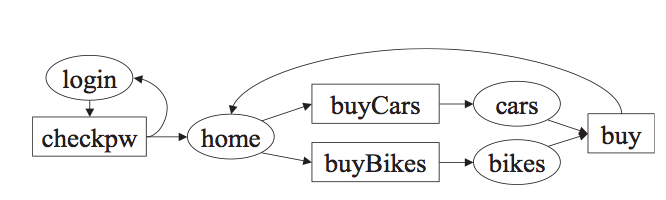
\includegraphics[width=11cm]{images/revangie-formchart.png}
			\caption{An example for a formchart. Related scenario is to be found in \cite{draheim2005source}}
			\label{revangie-formchart}
	\end{figure} 
	
	\begin{description}
		\item[\emph{Reverse Engineering Process}]\mbox{}\\ 
		Revangie has a complex way of analyzing web sites. It is using the form-oriented user interface model, which are graphs that contains all information about the pages and additionally relationships between server-side actions and pages. An example for a formchart diagram is Figure \ref{revangie-formchart}. The pages are obviously leading through different work flows but still have a common relationship to the page \emph{buy}. For more information about form-oriented analysis refer to \cite{draheim2005form}. 
		
		Based on that the Revangie algorithms provied three modes for gathering data from web sites:
		\begin{itemize}
			\item Crawl-mode\\
				An fully automatic mode, that acts like a HTTP bot that randomly navigates and enters values.
			\item Snoop-mode\\
				A data collecting mode, that needs actual users who maintain the session. More realistic data is gathered than with the crawling mode. 		
			\item Guide-mode\\
				A hybrid mode of the previous modes. 
		\end{itemize}
		
		\item[\emph{Comparison}]\mbox{}\\
		Revangie addresses many problems that Social Weaving has to deal with as well. Such issues like the \emph{screen classification} or \emph{targets identity} are topic in this thesis as well. The main difference to Social Weaving is that the whole web site code is being analyzed. Even though this leads to a better overview and the opportunity to generate models, the drawbacks for Social Weaving are immense as we see for the parameter DOM tree in Section \ref{param-dom-tree}.		
	\end{description}
\end{enumerate}

\newpage

\subsection{Use Cases}
The purpose of this section is to give the reader a clear idea about what functions our system should provide. Use cases are categorized for the plugin (or the client) and the server side. 

\begin{figure} \centering
		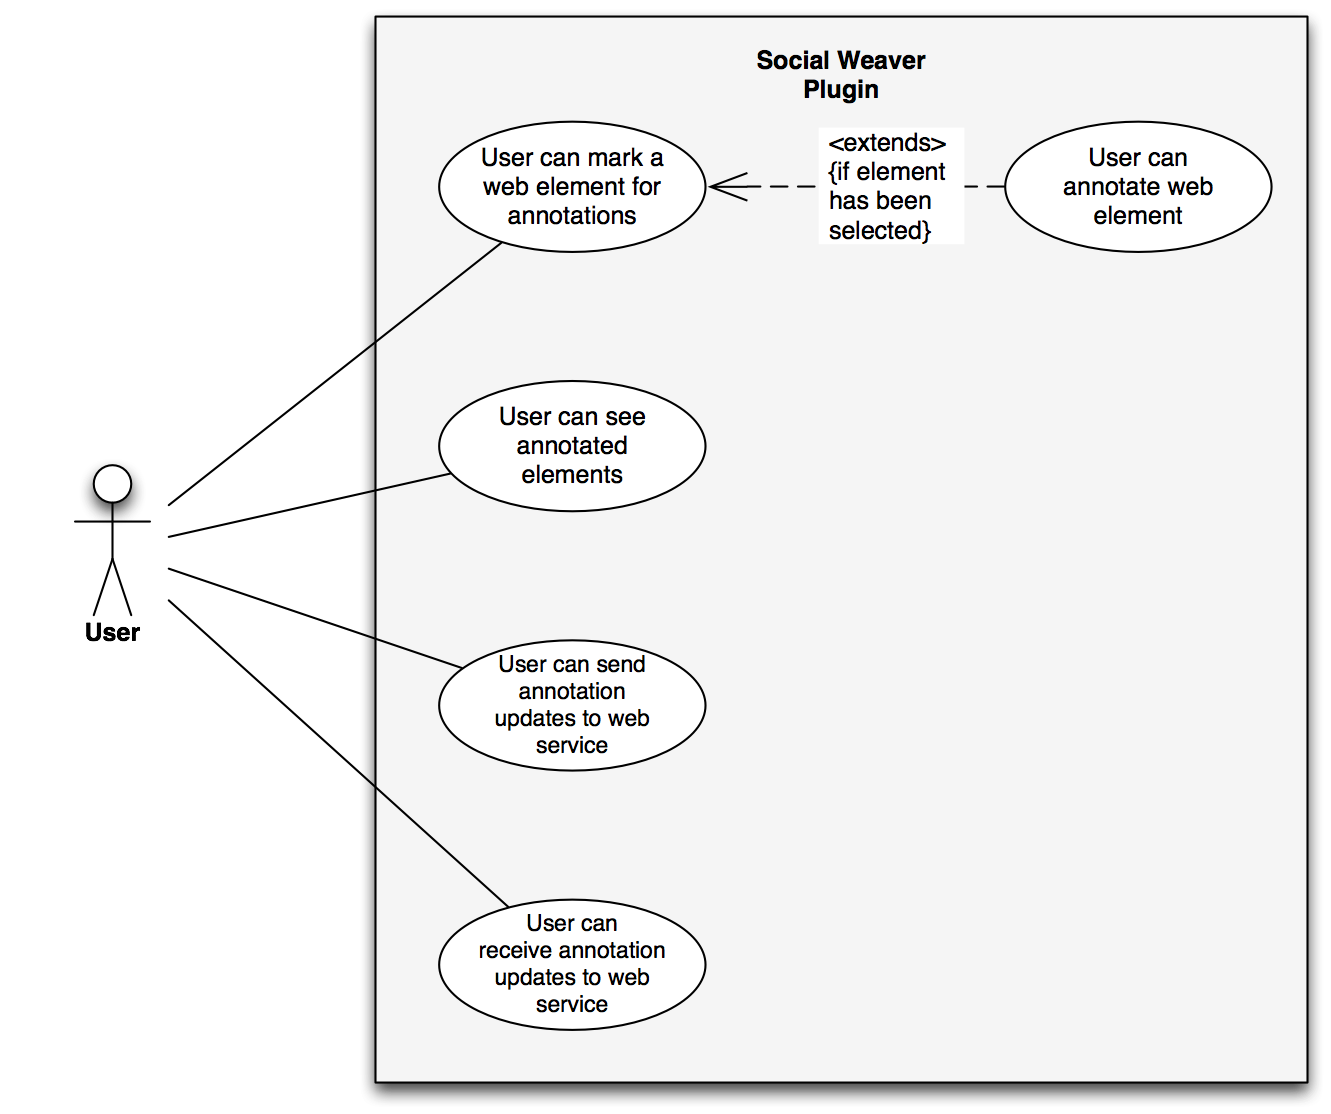
\includegraphics[width=13cm]{images/plugin-usecase-diagram.png}
		\caption{Use cases for the plugin}
		\label{plugin-usecase-diagram}
\end{figure} 


\begin{figure}\centering
		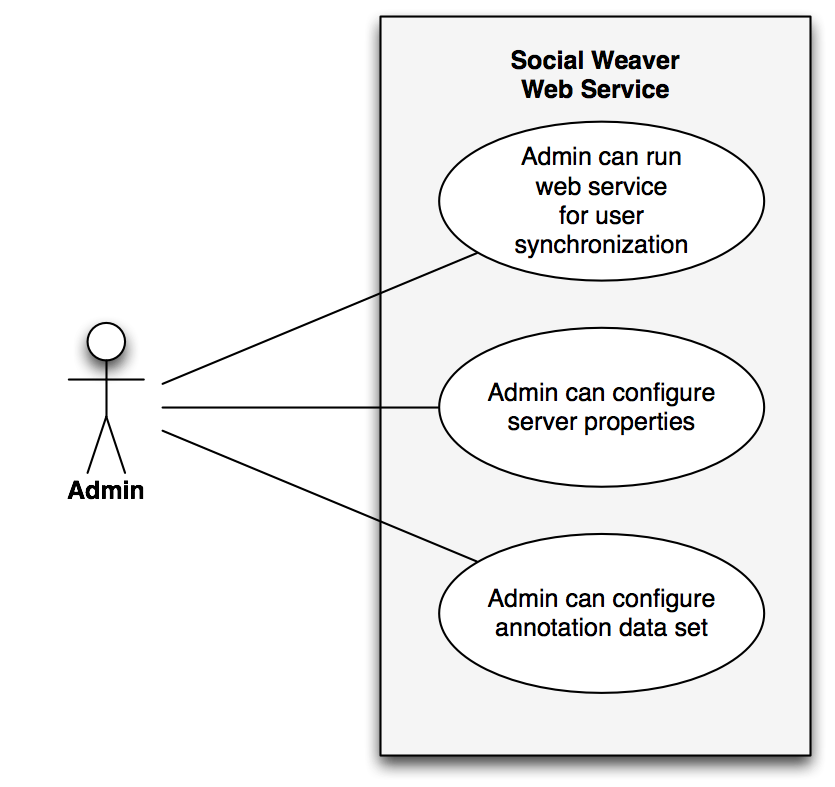
\includegraphics[width=8cm]{images/server-usecase-diagram.png}
		\caption{Use cases for the web service}
		\label{server-usecase-diagram}
\end{figure} 

\newpage
\subsection{What is Social Weaver}\label{what_is_sowe}
Social Weaver (SoWe) is the name of a prototype system that weaves social web features into web applications. The system consists of a Firefox plugin and the server side.

\begin{figure}\centering
		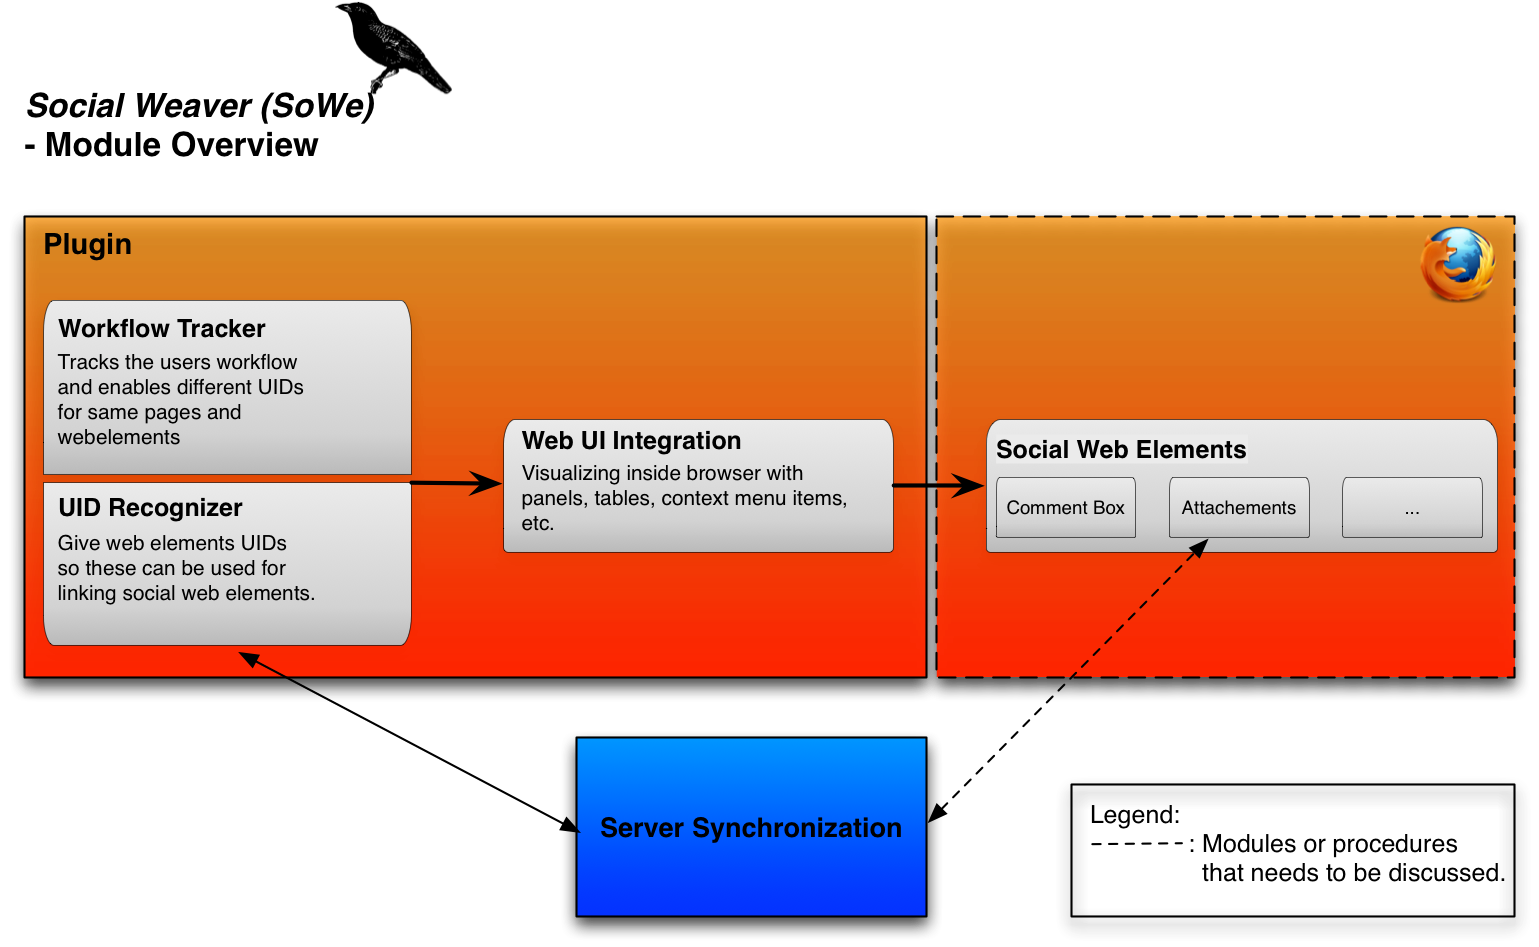
\includegraphics[width=13cm]{images/sowe-module-overview.png}
		\caption{Social Weaver Module Overview}
		\label{msowe-module-overview}
\end{figure} 

The plugin takes control of one or multiple user sessions and draws the additional content into the browser view. The server application synchronizes with each plugin and distributes updates between several clients. 

For a better understanding lets step through a generic use case where a user just opens a web application and modifies some content. The use case enumeration is related to the Figure \ref{sowe-prototype-use-case}.

\begin{enumerate}
\item The user opens a web application
\item The SoWe-Plugin sends a notification to the server with all necessary information like user identifier, time stamp, ...
\item After the server receives the plugin message it synchronizes it with its current content in the database
\item The server application responses to the plugin client with content data if some exists
\item The plugin uses the content information from the server to insert all social web elements
\item The user decides to make some changes to the social web content (e.g. adds a comment or creates a new comment box)
\item Again a notification is being sent to the server with containing the changes
\item Server synchronizes the updates and responses
\item Plugin redraws the synchronized content
\end{enumerate}

\begin{figure}\centering
		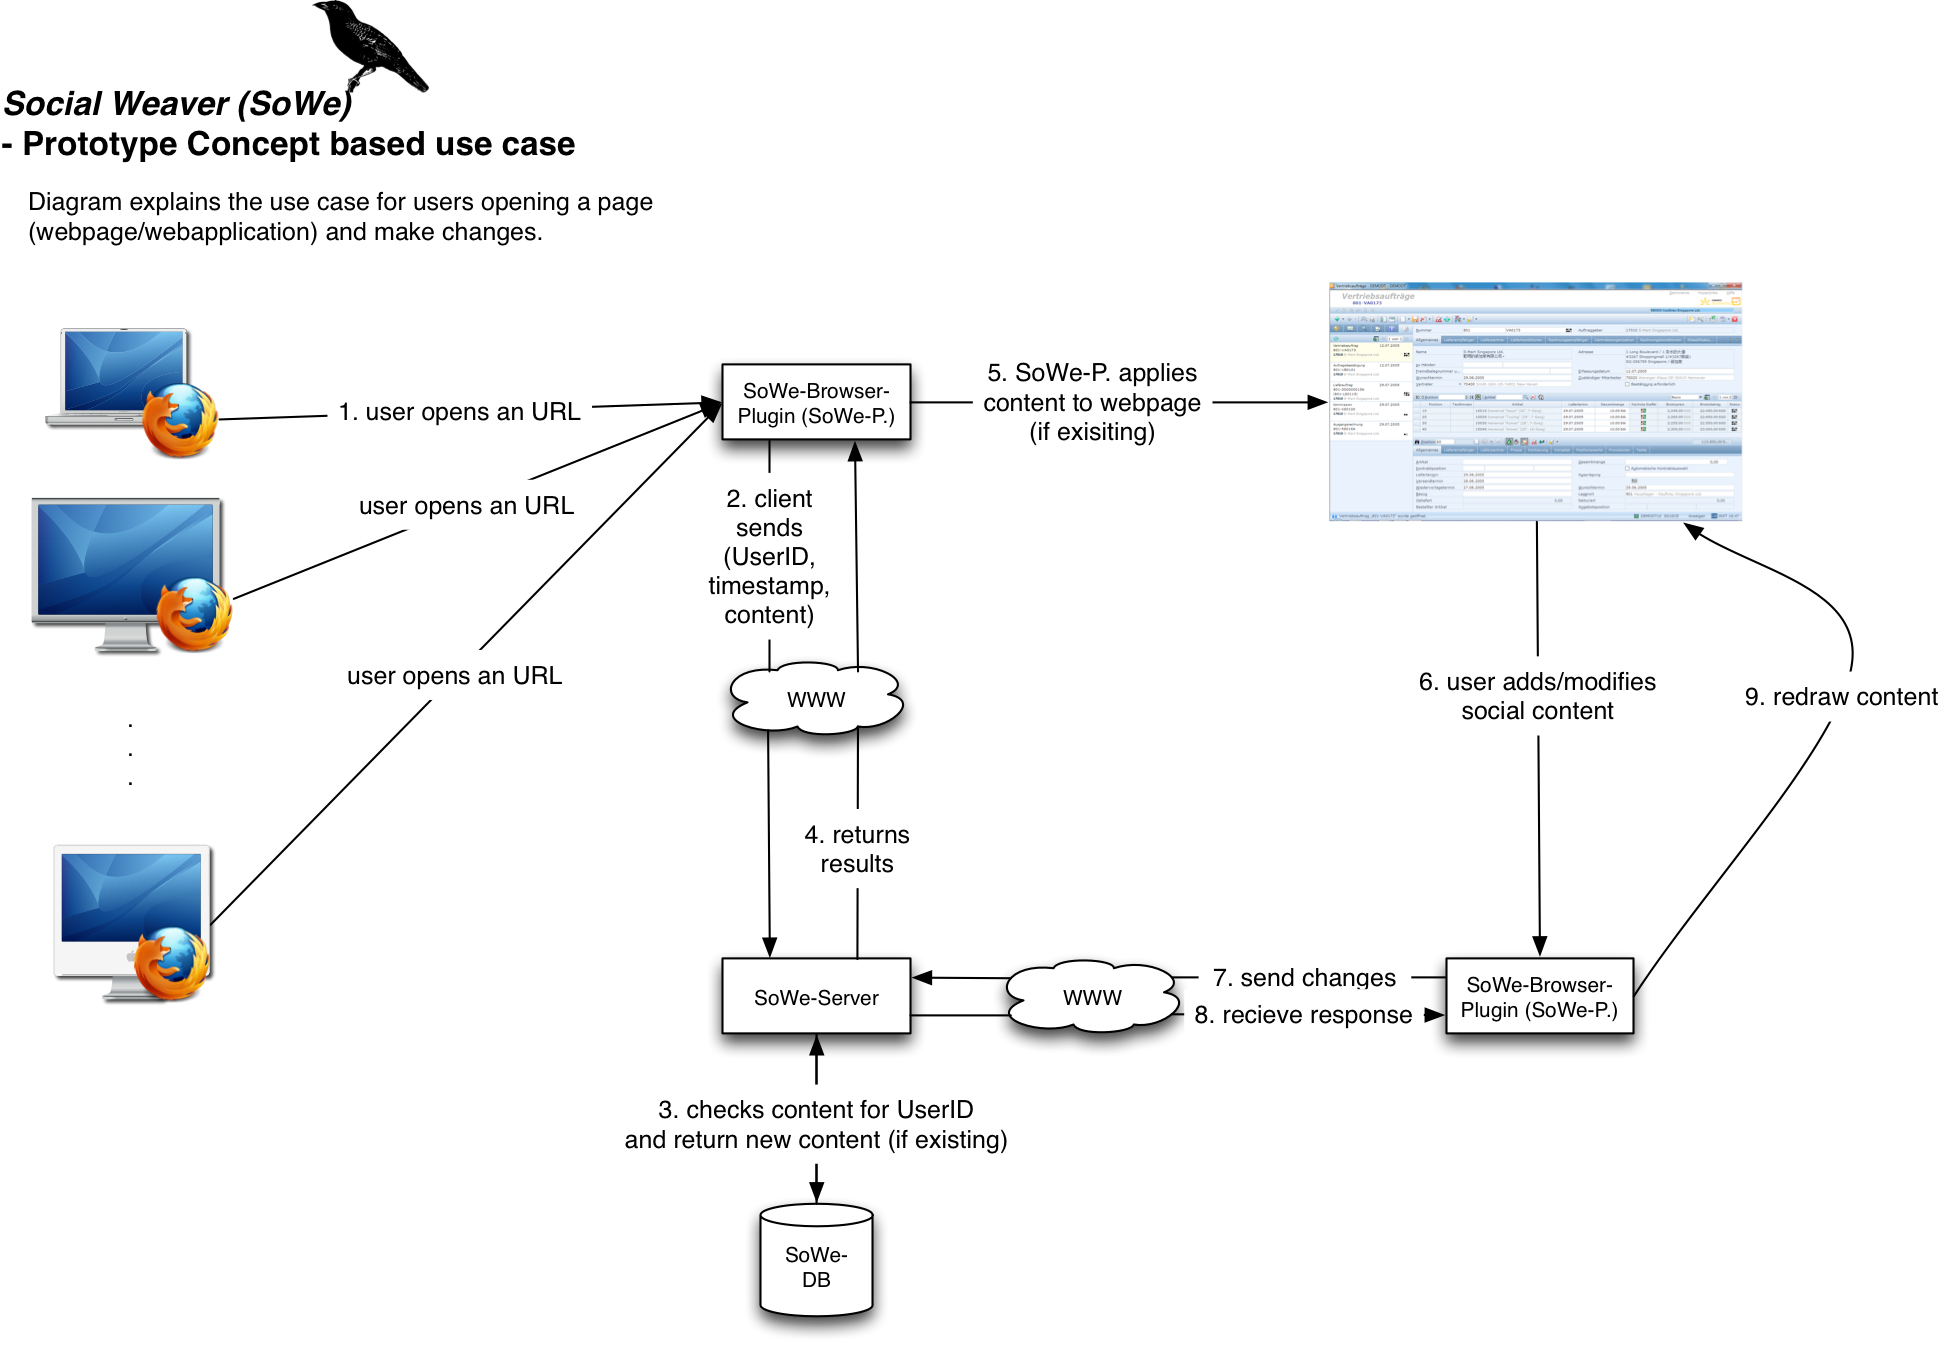
\includegraphics[width=13cm]{images/sowe-prototype-use-case.png}
		\caption{Social Weaver Prototype Use Case}
		\label{sowe-prototype-use-case}
\end{figure} 

\subsection{Requirements for Social Weaver}\label{sowe-reqs}

The general goal for Social Weaver is to weave social web 2.0 features into web-based applications. Since this is a broad requirement and impossible to be applied to any web application right from the beginning; it is necessary to break it down for the prototype.

More specifically the primary goal should be to get a system, that weaves one social web feature into a specific web application. Social Weaver has to be designed in a modular way, so that it is possible to add more social media features, support multiple platforms and more web applications. Now that we have a rough idea what SoWe is going to be, lets list some concrete high-level requirements:

\begin{enumerate}
\item Browser plugin that supports a comment box
\item Server application that stores and synchronizes data that it receives from different client-plugins
\item Data format for storing and processing data for social web content
\item Communication protocol between plugin and server
\end{enumerate}

With these requirements we can start to specify our enlisting in detail:

\subsubsection{Browser Plugin}\label{browser_plugin}
In the following we define requirements on concept level according to \cite{van2009requirements}. A specification to an implementation level follows in Section \ref{firefox_plugin_requirements}, where we have specified what technologies to use.

As already mentioned the main requirement is that the plugin supports a comment box. That means that the browser has to display a comment box that is related to specific web element. For example, in an online calendar an user adds a comment box related to an appointment that he wants to discuss in detail. 
Because it should be possible to add multiple comment boxes to any web element, we cannot just drop a box inside the user view, overlapping other interesting parts of the web application. Hence we have the requirement to make additional content visible to the user without interfering with the view on the original content. Possibilities would be fold/unfold-windows or just using small icons as references in the original view and outsource additional social content in external windows.

Of course the plugin needs to be able to communicate to the server application as well. (The server application is explained in the next Section \ref{Social Weaver - Server Application}). First of all the plugin needs to receive data that it print to the screen. Secondly changes made by the user has to be reported to the server. Because we are distributing the information between several users, there is also a need for synchronization. User updates may not overwrite updates made by other users etc.

The parser framework contains application programming interfaces that create and parse the content of our tuples. This way it is, for instance, easier to add plugins for other browsers. 
The data in the content-part of our tuple should have a uniform format no matter what web application or browser is in use. The server application doesn't need to be aware about the environment the plugin runs in - it manages the social web content independently.

Another tricky and important point is the interaction with the web application. Most such sites are dynamic and there exists no static URLs we can refer to. And it is not certain that the same element, that two users refer to in their independent sessions, has a comparable identifier. This issue definitely needs to be handled specifically for any web application. The good news is that this only affects the plugin. The server application just needs clearly defined identifiers. As a solution for the plugin we need the possibility to use scripts for identifying elements. For example, a script that supports the Google calendar is injected to make the plugin identify same appointments in different user sessions. This requirement is probably the vastly problematic one because it prevents a general usage of Social Weaver.

Lets summarize all the requirements we gained in this section:

\begin{enumerate}
\item \reqPi
\item \reqPii
\item \reqPiii
\item \reqPiv
\item \reqPv
\item \reqPvi
\item \reqPvii
\end{enumerate}

\subsubsection{Server Application} \label{Social Weaver - Server Application}
The server applications primary requirement is to synchronize different user sessions on one or multiple web applications. A user session is defined within the plugin (which doesn't mean a plugin can manage only one session). The server basically receives messages from different sessions, synchronizes them and distributes the most current state to all sessions.  To establish a loss less synchronization every message contains a time stamp.

We are assuming that every message contains an user identifier, a time stamp and an unique identifier for an element within the web application. This Anchor is the unique identifier for a single user action. For example, if a user adds a comment to an already existing comment box that is related to an appointment in a calendar, the server receives the users identifier, the time stamp for the modification and an identifier for the appointment in the calendar. With this information the server can check its database for the comment box and add the new comment. 

It is important to remember that the server only uses the received data as identifier. All actions are completely independent to the web application. 

Also we may assume that the received message have the same Anchor form as discussed in the previous section. 
\begin{verbatim}(user identifier, time stamp, content)\end{verbatim} 
The content part from the Anchor needs to be in an uniform format that has been generated by the plugin. So even the browser type doesn't matter to the server. The server has to be able to parse the content package and to create a new one that can be parsed by our plugins.

So the requirements for the server application are:
\begin{enumerate}
\item \reqWSi
\item \reqWSii
\item \reqWSiii
\item \reqWSiv
\item \reqWSv
\item \reqWSvi
\item \reqWSvii
\end{enumerate}

\subsubsection{Social Weaver - Script Support} \label{abstract-script-support-reqs}
The support for external scripts is essential for a generic usage of Social Weaver. The reason why script support is extracted into its own section, is that it should be decoupled from the server and plugin that were discussed before. 

The underlying problem is the problematic identification of elements of a web view. There is simply no generic way of identifying elements in the users view across all web sites and applications. For that reason we need an extendable method to support more websites and applications. This could even mean that third-parties could support their own systems by just adding the script without the need to modify Social Weaver directly. In this section we briefly discuss what the purpose of such scripts is in detail and what requirements we have to fulfill. 
\\ \\
The term \textit{script} in our context should contain only information that is needed by the plugin to identify an element. Let us consider the Google calendar example once again. The case where we want to match the same appointment field across different user sessions brings the problem that there is no identifier for the element itself. To the user it is obvious to identify it because of the appointment name, date and time. And those parameters could be just the information we need to extract into our script. How this looks like in detail is discussed in the implementation level section. 

The usage of scripts should be related to one or a set of URLs. This affects mostly the root URL of a server. But might be used for sub parts of a web page or application. As example a script related to \textit{http://www.opensource.org/} is applied to all sub pages like \textit{http://opensource.org/docs/board-annotated}. 

But it might be of use to have a special matching procedure for sub pages.  In that case a script for \textit{http://opensource.org/faq} would overwrite the more general script. 

A set of URLs could be used for scripts that are applicable for many websites. 

The work flow when a script is used and when the default matching procedure that comes with the plugin is quite straightforward (see Figure \ref{script-usage-basic}). When opening a new URL then the plugin should check whether there is a script for that case and depending on the search results proceed with the script or default matching procedure.

\begin{figure}\centering
		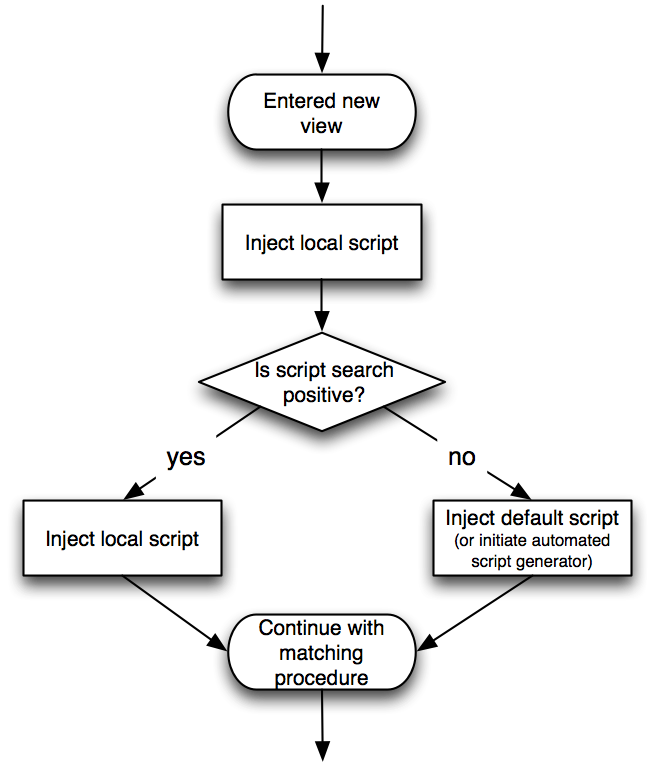
\includegraphics[width=7cm]{images/script-usage-basic.png}
		\caption{Work flow for Script Using}
		\label{script-usage-basic}
\end{figure} 

On the conceptual level we have the following requirements:

\begin{enumerate}
\item \reqSi
\item \reqSii
\item \reqSiii
\item \reqSiv
\item \reqSv
\item \reqSvi
\end{enumerate}
